\documentclass[tikz,border=5mm]{standalone}
\usetikzlibrary{calc}
\begin{document}
	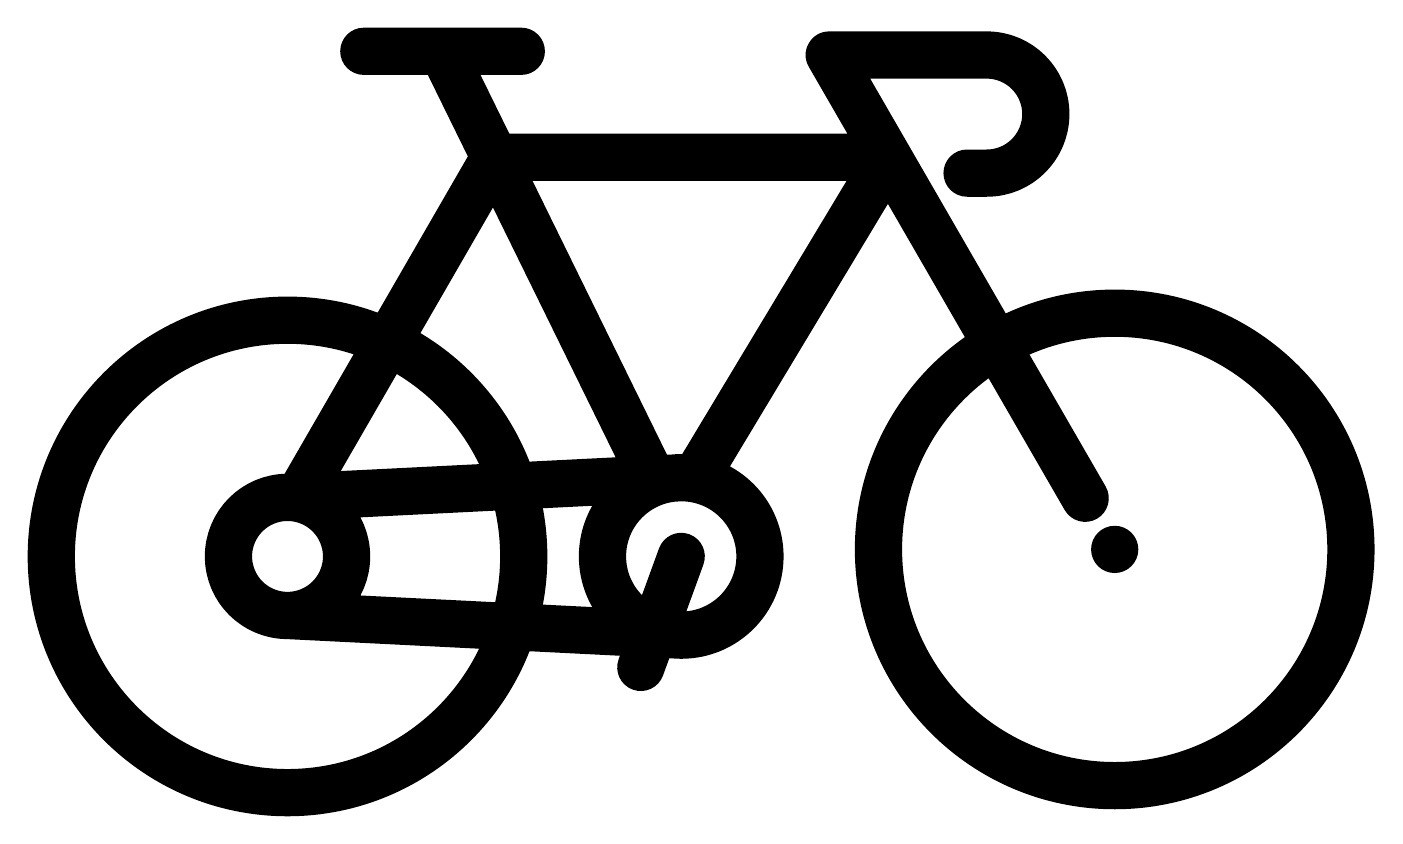
\begin{tikzpicture}
		\draw[line width=6mm,join=round,cap=round]
		(0:0) circle (.75)
		(0:0) circle (3)
		(90:.75) arc (90:270:.75) --(5,-1) arc (-90:90:1)--cycle
		(5,0) circle (1)
		(5,0)--++(-110:1.5)
		(80:.75)--++(60:5) coordinate (A)--++(0:5) coordinate (B)--++(-60:5) coordinate (C)
		(C)++(-60:.75) circle (3)
		(5,0)+(110:1)--(A)--([turn]0:1.5) coordinate (D)
		(5,0)++(80:1)--(B)
		(D)++(180:1)--++(0:2)
		(C)--(B)--([turn]0:1.5)--++(0:2) arc (90:-90:.75)--++(180:.25);
		\fill (C)++(-60:.75) circle (.3);
	\end{tikzpicture}
\end{document}